
\Formula{A$_{\bm4}$}{
	设
	\Equation{
		f\braI{x}=\arctan\frac{1+x}{1-x}\ ,
	}
	计算 $f\fnder{2n}\braI{0}$ , 其中 $n\in\bfN$ .
}
\Proof{证明I\score{1}}{
	\par 注意到 $x<1$ 时有 $f\braI{x}-\sfrac{\pi}{4}=\arctan x$ 是奇函数, 因此 $f\braI{x}$ 在 $x=0$ 处的任意正偶数阶导数均为 $0$ , 即
	\Equation{
		f\fnder{2n}\braI{0}=\boxed{\casesII{\sfrac{\pi}{4}}{n=0}{-2}{0}{n\ne 0}}\ .
	}
	\begin{center}
		\begin{tikzpicture}
    		\begin{axis}[
        		width = 12cm,
        		height = 7cm,
        		xmin = -3.5, xmax = 3.5,
        		ymin = -2.25, ymax = 2.25,
        		xtick = {-3, -2, -1, 0, 1, 2, 3},
        		ytick = {-1.5708, -0.7854, 0, 0.7854, 1.5708},
        		yticklabels = {$-\sfrac{\pi}{2}$, $-\sfrac{\pi}{4}$, $0$, $\sfrac{\pi}{4}$, $\sfrac{\pi}{2}$},
        		axis lines = middle,
        		legend pos = north west,
        		legend cell align = {left},
				legend style={
        			draw = white,
        			inner sep = 0pt,
        			minimum height = 0.5cm,
        			font = \small
    			}
    		]
    		\addplot[
        		domain = -4.5:4.5,
        		samples = 100,
        		color = blue,
        		thick
    		]{rad(atan(x))};
    		\addlegendentry{\ $y=\arctan x$}
    		\addplot[
        		domain = -4.5:0.95,
        		samples = 100,
        		color = red,
        		thick
    		]{rad(atan((1+x)/(1-x)))};
    		\addlegendentry{\ $y=f\braI{x}$}
    		\addplot[
        		domain = 1.05:4.5,
        		samples = 100,
        		color = red,
        		thick,
    		]{rad(atan((1+x)/(1-x)))};
    		\end{axis}
		\end{tikzpicture}
	\end{center}
}
\Proof{证明II\score{0.5}}{
	\par 在 $\braI{-1\and 1}$ 上应用逐项积分可得
	\Equation{
		\arctan x&=\Int{0}{x}{\frac{1}{1+t^{2}}}{t}\\[1mm]
		&=\Int{0}{x}{\sum_{n=0}^{\infty}\braI{-1}^{n}t^{2n}}{t}\\[1mm]
		&=\sum_{n=0}^{\infty}\Int{0}{x}{\braI{-1}^{n}t^{2n}}{t}\\[1mm]
		&=\sum_{n=0}^{\infty}\frac{\braI{-1}^{n}x^{2n+1}}{2n+1}\ ,
	}

\newpage

	\noindent 于是 $\braI{\arctan x}^{(2n)}\subst{x=0}{}=0$ , 又由 $f\braI{x}=\sfrac{\pi}{4}+\arctan x$ 可知
	\Equation{
		f\fnder{2n}\braI{0}=\boxed{\casesII{\sfrac{\pi}{4}}{n=0}{-2}{0}{n\ne 0}}\ .
	}
}
\Proof{$^{*}$证明III\score{0.5}}{
	\par 当 $n=0$ 时, 我们有 $f\braI{0}=\sfrac{\pi}{4}$ .
	\par 当 $n\ne 0$ 时, 我们有
	\Equation{
		\braI{\arctan\frac{1+x}{1-x}}^{(2n)}&=\braI{\frac{1}{x^{2}+1}}^{(2n-1)}\\[2mm]
		&=\frac{1}{2\rmi}\braII{\!\braI{\frac{1}{x-\rmi}}^{(2n-1)}-\braI{\frac{1}{x+\rmi}}^{(2n-1)}}\\[1mm]
		&=\frac{\braI{2n-1}\,!}{2\rmi}\braI{\frac{1}{\braI{x+\rmi}^{2n}}-\frac{1}{\braI{x-\rmi}^{2n}}}\ ,
	}
	此时 $f\fnder{2n}\braI{0}=0$ .
	\par 综上所述, 我们有
	\Equation{
		f\fnder{2n}\braI{0}=\boxed{\casesII{\sfrac{\pi}{4}}{n=0}{-2}{0}{n\ne 0}}\ .
	}
}
\Proof{要点}{
	+ 解法I使用了如下关于反正切函数 $\arctan$ 的恒等式:
	\Equation{
		\arctan x+\arctan y=\casesIII{\arctan\frac{x+y}{1-xy}}{xy<1}{1}{\arctan\frac{x+y}{1-xy}+\pi}{xy>1\text{且}x>0}{1}{\arctan\frac{x+y}{1-xy}-\pi}{xy>1\text{且}x<0}\ .
	}
	+ 解法III需要将 $f$ 延拓至 $\bfC$ 中, $\bfR$ 中绝大多数导数相关的结论在 $\bfC$ 中依然成立.
	+ 对于反正切函数 $\arctan$ , 我们有如下泰勒公式成立:
	\Equation{
		\arctan x=\sum_{k=0}^{n}\braI{-1}^{k}\frac{x^{2k+1}}{2k+1}+R_{n}\braI{x}\ .
	}
}

\newpage

\Formula{B$_{\bm4}$}{
	设
	\Equation{
	    f\braI{x}=\braI{x^{3}-1}^{n}\arctan x\ ,
	}
	计算 $f\fnder{n}\braI{1}$ , 其中 $n\in\bfN$ .
}
\Proof{证明\score{1.5}}{
	\Equation{
		&\hphantom{=\,}\braI{\!\braI{x^{3}-1}^{n}\arctan x}^{(n)}\subst{x=1}{}\\[1mm]
		&=\sum_{k=0}^{n}\rmC_{n}^{k}\braI{\!\braI{x-1}^{n}}^{(n-k)}\braI{\!\braI{x^{2}+x+1}^{n}\arctan x}^{(k)}\\[1mm]
		&=n\,!\braI{x^{2}+x+1}^{n}\arctan x+\sum_{k=1}^{n}\rmC_{n}^{k}\underbrace{\braI{\!\braI{x-1}^{n}}^{(n-k)}}_{x=1\text*{时为}0}\braI{\!\braI{x^{2}+x+1}^{n}\arctan x}^{(k)}\ ,
	}
	于是
	\Equation{
		f\fnder{n}\braI{1}=\boxed{\frac{3^{n}n\,!}{4}\pi}\ .
	}
}
\Proof{要点}{
	+ $\braI{x-a}^{n}$ 当且仅当在 $n$ 阶导后化为常数, 使用Leibniz公式时需要注意利用这一性质.
}

\bigskip

\Formula{C$_{\bm4}$}{
	设
	\Equation{
	    f\braI{x}=\frac{\arcsin x}{\sqrt{1-x^{2}}}\ ,
	}
	计算 $f\fnder{2n+1}\braI{0}$ , 其中 $n\in\bfN$ .
}
\Proof{证明\score{2}}{
	\par 等式两侧同时乘 $\sqrt{1-x^{2}}$ 并对其求导, 我们有
    \Equation{
        f\fder\braI{x}\sqrt{1-x^{2}}-\frac{xf\braI{x}}{\sqrt{1-x^{2}}}=\frac{1}{\sqrt{1-x^{2}}}\ ,\\[-15mm]
    }
    \Equation{
        \braI{1-x^{2}}f\fder\braI{x}=xf\braI{x}+1\ ,
    }
    再对等式两侧同时求 $n-1$ 阶导, 我们有
    \Equation{
        \braI{1-x^{2}}f\fnder{n}\braI{x}-\braI{2n-1}xf\fnder{n-1}\braI{x}-\braI{n-1}^{2}f\fnder{n-2}\braI{x}=0\ ,
    }

\newpage

    \noindent 代入 $x=0$ 时即得 $f\fnder{n}\braI{0}=\braI{n-1}^{2}f\fnder{n-2}\braI{0}$ , 由 $f\fder\braI{0}=1$ 即得其通项公式
    \Equation{
        f\fnder{2n+1}\braI{0}=\boxed{\braI{\!\braI{2n}\,!!}^{2}}\OR f\fnder{2n+1}\braI{0}=\boxed{4^{n}\braI{n\,!}^{2}}\ ,
    }
	其中我们规定 $0\,!!=1$ .
}
\Proof{要点}{
	+ 我们可以将 $n$ 阶导数 $f\fnder{n}$ 视作函数列, 并通过构造递推公式来计算其通项公式, 常见的做法是构造以 $f$ 为特解的简单线性微分方程, 然后对等式两侧同时求 $n$ 阶导.
}

\newpage
